%!TEX root=document.tex

\section{Qualitative Study}\label{sec:example-viz}

In this section, we study some examples of visualizations recommended and
not recommended by \VizRecDB for real-world datasets.
We once again turn to the BANK and DIAB datasets described in 
Section~\ref{sec:experiments}.

We first consider the DIAB dataset. 
The query selects a group of diabetes patients in the age range 30--40;
these patients are compared against all patients.
In Figure~\ref{fig:qual-study}, we list one example of a visualization
that is recommended by \VizRecDB, and one that is not recommended by \VizRecDB.
We acknowledge that the charts outputted by \VizRecDB could look prettier and be better
formatted to make the output more usable and interpretable; this has not been our focus thus far. 
We plan to address these presentation issues in the future.

The visualization recommended by \VizRecDB (Figure~\ref{fig:time-in-hospital}) has utility 0.174 (via
the Earth Mover's Distance utility metric).
This visualization depicts the time in hospitals spent by
individuals of different race, for the selected patients
(i.e., those between 30 and 40), and
the rest. 
As can be seen in this figure, this visualization is indeed interesting;
when we compare the average amount of time spent in hospital 
for african americans and caucasians, 
for the selected patients, the amount of time spent in hospital
by african americans and caucasians is quite close to each other,
while across all age groups, caucasians spend a lot more time
in hospital.

The visualization not recommended by \VizRecDB (Figure~\ref{fig:lab-procedures}) has utility 0.004, very close to 0.
This visualization depicts the fraction of patients that 
have either had or not had lab procedures. 
As can be seen in the figure, the same fraction of patients in
both the selected patients as well as all patients
have had lab procedures.
This is therefore not as interesting a visualization.

As can be seen, 
the visualizations produced by \VizRecDB based on the Earth Mover's Distance
metric ends up giving useful, interesting visualizations on two of
the real world datasets we have experimented with.



\begin{figure}[h] 
\centering
\begin{subfigure}{0.8\linewidth}
\centering
{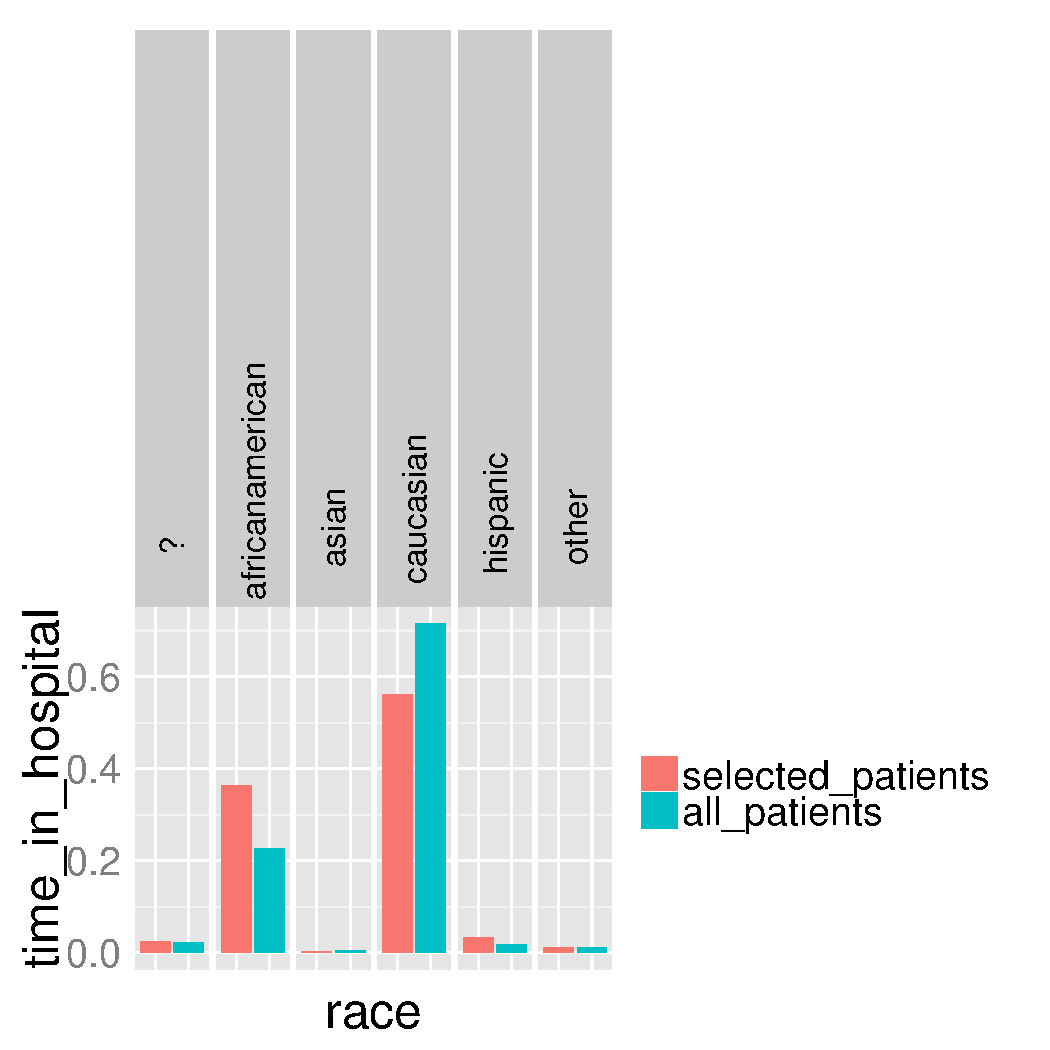
\includegraphics[width=7cm] {Images/seedb_dim_race_measure_time_in_hospital.pdf}}
\caption{Time in Hospital by Race: Recommended by \VizRecDB}
\label{fig:time-in-hospital}
\end{subfigure}
\begin{subfigure}{0.8\linewidth}
\centering
{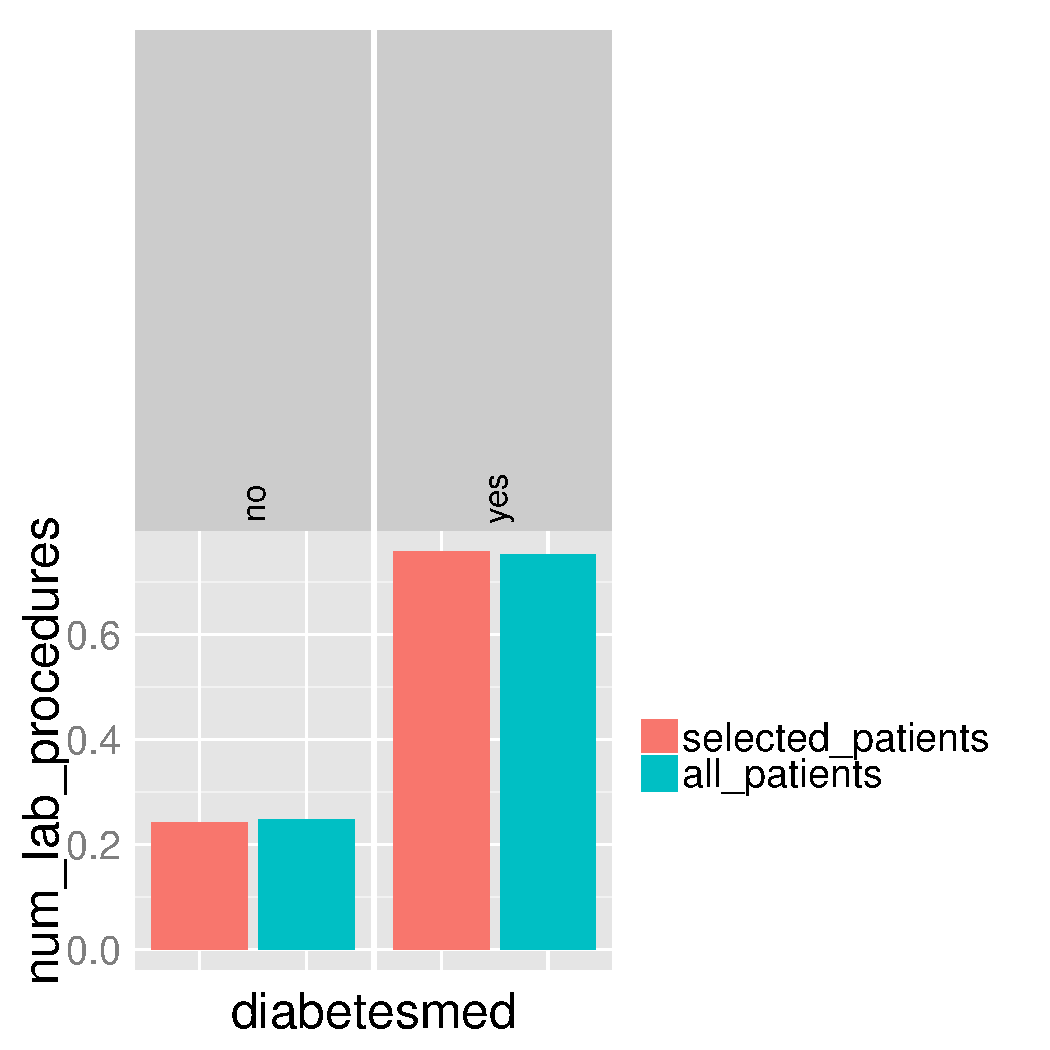
\includegraphics[width=7cm] {Images/seedb_dim_diabetesmed_measure_num_lab_procedures.pdf}}
\caption{Lab Procedures: Not Recommended by \VizRecDB}
\label{fig:lab-procedures}
\end{subfigure}
\vspace{-10pt}
\caption{\VizRecDB Generated Visualizations}\label{fig:qual-study}

\vspace{-10pt}
\end{figure}

